\begin{frame}
 \frametitle{Оптимизация}
 \begin{itemize}
  \item Преждевременная оптимизация -- корень всех зол!
  \pause
  \item Закон Амдала
     \begin{equation*}
        \frac{1}{(1-P)+\alpha P}
     \end{equation*}
  \item Профилирование -- выясним, в каких местах программа проводит больше всего времени
 \end{itemize}
\end{frame}

\begin{frame}
    \frametitle{Профилирование в Linux}
    \center
    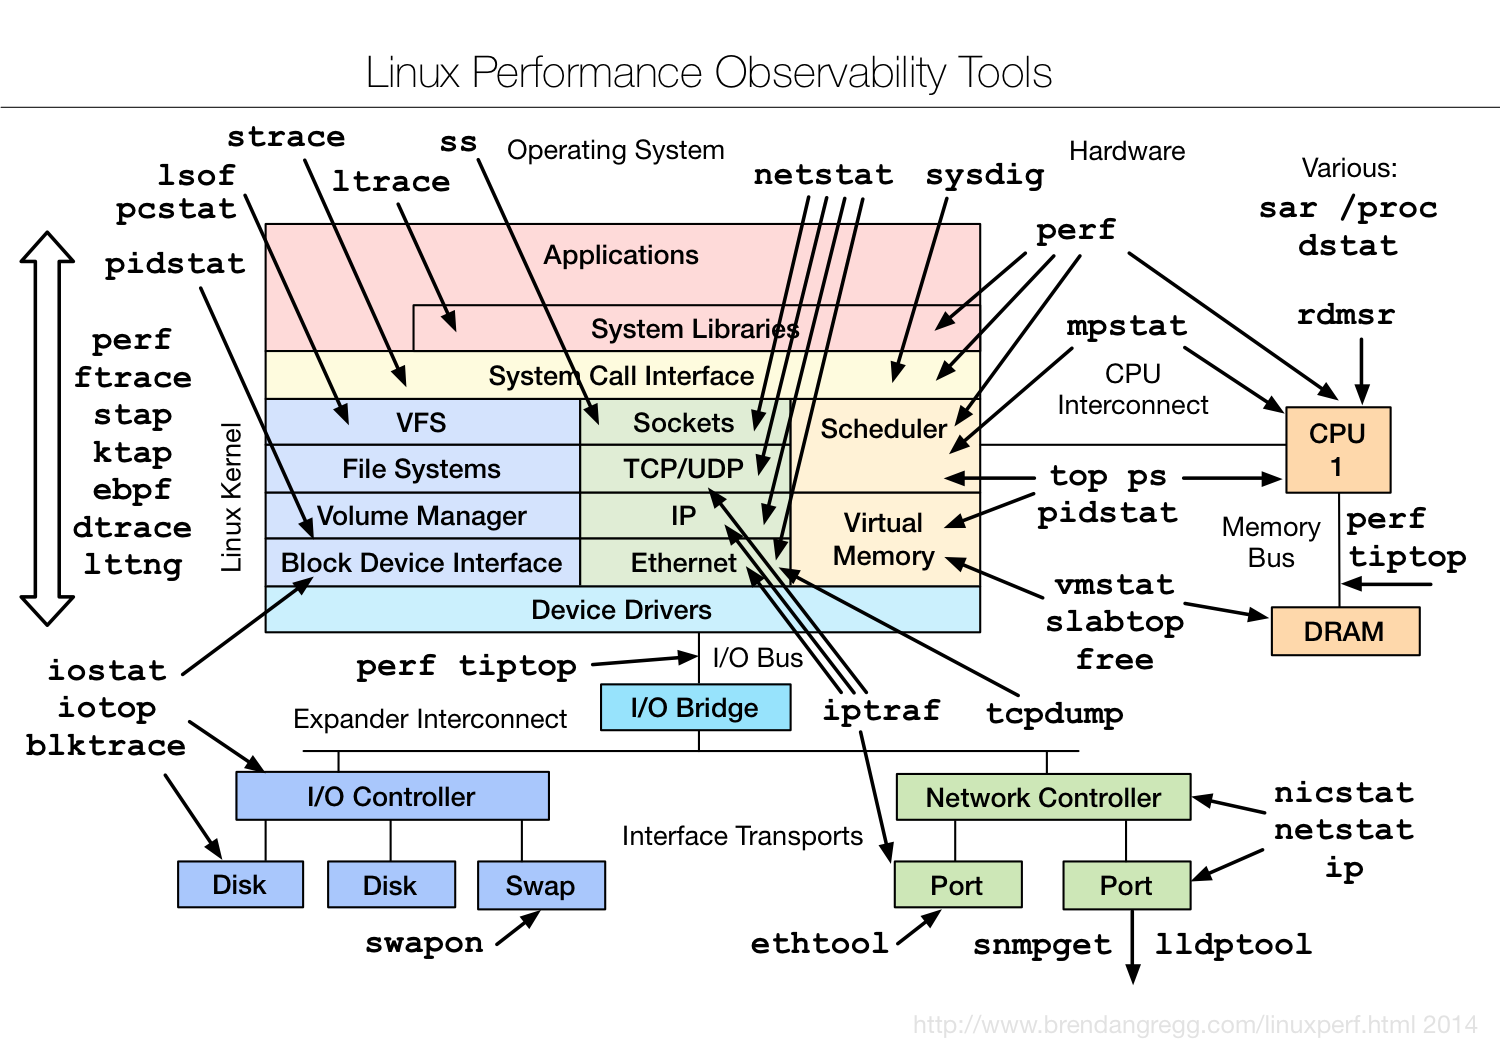
\includegraphics[height=0.75\textheight]{../../slides/profile/linux_observability_tools.png}\footnote{\url{http://www.brendangregg.com/linuxperf.html}}

\end{frame}


\begin{frame}
  \frametitle{Методы профилирования}
  \begin{itemize}
    \item Добавление в код дополнительных инструкций (gprof)
      \begin{enumerate}
        \item[Достоинства] Не требуется поддержка ядра
        \item[Недостатки] Рекомпиляция, замедление кода
      \end{enumerate}
    \item Статистическое исследование (oprofile,perf)
      \begin{enumerate}
        \item[Достоинства] Малое вмешательство в процесс, скорость
        \item[Недостатки] Требуется модуль ядра, точность
      \end{enumerate}
    \item Эмуляция процессора для перехвата вызовов (valgrind)
       \begin{enumerate}
         \item[Достоинства] Не требуется рекомпиляция и модули ядра
         \item[Недостатки] Скорость
        \end{enumerate}
    \item Перехват системных и библиотечных вызовов (strace,ltrace)
       \begin{enumerate}
          \item[Достоинства] Нет рекомпиляции, любое ядро
          \item[Недостатки] Недостаточная информативность
       \end{enumerate}
  \end{itemize}
\end{frame}

